\section{Results}
All holdout estimates come from a single run of the frozen specification; secondary tests are labelled exploratory. The development column uses the corrected release times (Section~\ref{sec:amend}). Standard errors are clustered by year (seven clusters), so we report wild cluster bootstrap $p$-values alongside.

\paragraph{Primary holdout test.} Table~\ref{tab:primary} reports the primary specification. The anxious-state premium is 37.8~bps ($t=1.91$, wild $p=0.149$) against 12.6~bps in development; its sign matches development but it does not reject zero at 5\%. The key contrast $b$ (anxious minus calm) is $-2.6$~bps (wild $p=0.946$): it does not replicate the development difference of 19.2~bps (wild $p=0.057$). The reason is the calm cell, whose mean rises from $-6.6$ to 40.4~bps. That cell has only nine meetings, so $b$ is weakly identified (Figures~\ref{fig:scatter} and~\ref{fig:state}). The continuous VIX slope is 5.02~bps per point ($t=2.48$) against 1.87 in development, but it is a single-sample, seven-cluster estimate and two high-VIX meetings in 2020 are visible leverage points in Figure~\ref{fig:scatter}. The matched-VIX placebo on non-meeting days gives a Fed-minus-matched difference of 55.5~bps ($p=0.002$) for all meetings and 38.3~bps ($p=0.030$) for anxious meetings, so the window return around meetings exceeds that on comparable non-meeting days. In development the same placebo shows no Fed-specific premium ($-11.9$~bps, $p=0.65$).

\begin{table}[ht]\centering\caption{Primary specification, development and holdout. Standard errors (year-clustered) in parentheses. Placebo sample sizes shown are for the holdout; development has 77, 38 and 39 meetings.}\label{tab:primary}
\small\begin{tabular}{lrr}\toprule
 & Development (corrected) & Holdout \\ \midrule
Calm mean $a$ (bps) & $-6.6$ (3.3) & 40.4 (5.4) \\
Anxious$-$calm $b$ (bps) & 19.2 (8.3) & $-$2.6 (21.9) \\
Anxious premium $a+b$ (bps) & 12.6 (7.5) & 37.8 (19.8) \\
Wild-bootstrap $p(b=0)$ & 0.057 & 0.946 \\
Wild-bootstrap $p(a+b=0)$ & --- & 0.149 \\
VIX slope $c$ (bps/pt) & 1.87 (1.05) & 5.02 (2.02) \\
\midrule
Placebo (all, $n=52$): Fed$-$matched (bps) & $-$11.9 ($p=0.65$) & 55.5 ($p=0.002$) \\
Placebo (anxious, $n=43$): Fed$-$matched (bps) & $-$12.0 ($p=0.81$) & 38.3 ($p=0.030$) \\
Placebo (calm, $n=9$): Fed$-$matched (bps) & $-$10.8 ($p=0.59$) & 35.2 ($p=0.209$) \\
\bottomrule\end{tabular}\end{table}

\begin{figure}[ht]\centering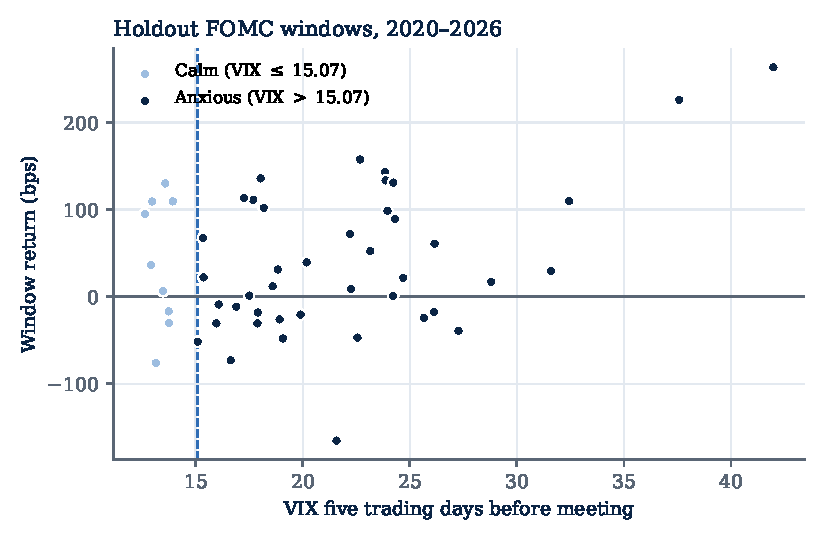
\includegraphics[width=.8\linewidth]{figures/fig1_holdout_scatter.pdf}\caption{Holdout meeting-window returns against lagged VIX.}\label{fig:scatter}\end{figure}
\begin{figure}[ht]\centering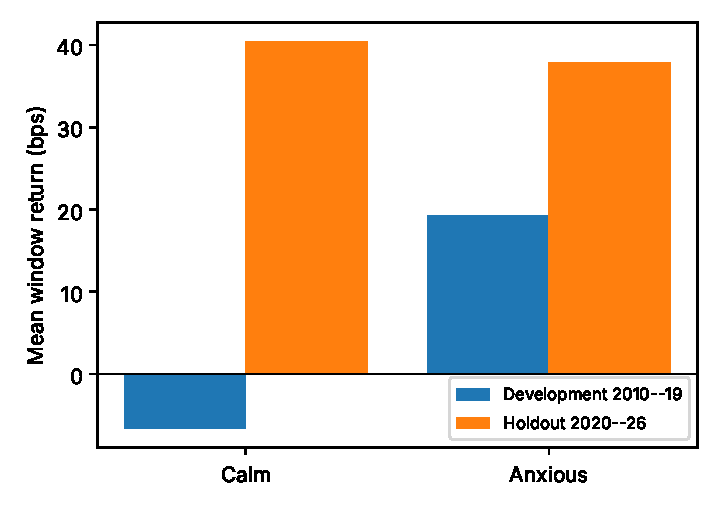
\includegraphics[width=.6\linewidth]{figures/fig2_state_means.pdf}\caption{Mean window return by state, development versus holdout.}\label{fig:state}\end{figure}

\paragraph{Exploratory secondary tests.} The VIX-change test finds no effect: the slope on the five-day VIX change is $-3.39$ ($t=-0.47$, wild $p=0.876$). The press-conference subsample (45 meetings from 2021 on) gives an anxious premium of 28.3~bps (wild $p=0.221$). The Federal Reserve held a press conference at every 2020 meeting too, which we verified only after the single run, so the subsample excludes 2020 for that reason; since the indicator equals one for all 52 holdout meetings, the subsample test adds nothing beyond the primary result and no comparison with non-press meetings is possible. Table~\ref{tab:robust} shows the anxious premium across thresholds, leave-one-year-out samples, winsorizing and no risk-free adjustment. It ranges from 26.6 to 69.5~bps. No wild $p$-value falls below 0.05, and the smallest is 0.092.

\begin{table}[ht]\centering\caption{Robustness of the holdout anxious premium (exploratory).}\label{tab:robust}
\small\begin{tabular}{lrrrrr}\toprule
Specification & $n$ & $n_{\mathrm{anx}}$ & Prem. (bps) & s.e. & Wild $p$ \\ \midrule
press=1 anxious premium & 45 & 37 & 28.3 & 20.5 & 0.221 \\
2021+ (flag-known sample) & 45 & 37 & 28.3 & 20.5 & 0.221 \\
baseline thr 15.07 & 52 & 43 & 37.8 & 19.8 & 0.149 \\
threshold 18 & 52 & 30 & 51.6 & 20.7 & 0.092 \\
threshold 20 & 52 & 23 & 59.2 & 22.3 & 0.194 \\
threshold 25 & 52 & 9 & 69.5 & 30.4 & 0.51 \\
holdout-median threshold & 52 & 26 & 48.7 & 25.2 & 0.284 \\
drop 2020 & 45 & 37 & 28.3 & 20.5 & 0.221 \\
drop 2021 & 44 & 35 & 51.9 & 17.2 & 0.114 \\
drop 2022 & 44 & 35 & 26.6 & 20.4 & 0.256 \\
drop 2023 & 44 & 39 & 41.6 & 21.7 & 0.199 \\
drop 2024 & 44 & 39 & 34.8 & 21.9 & 0.251 \\
drop 2025 & 44 & 35 & 37.7 & 24.7 & 0.3 \\
drop 2026 & 47 & 38 & 43.8 & 21.6 & 0.111 \\
excl 2020 (covid) & 45 & 37 & 28.3 & 20.5 & 0.221 \\
winsorized 5/95 & 52 & 43 & 35.9 & 16.2 & 0.121 \\
no rf adjustment & 52 & 43 & 38.8 & 19.8 & 0.135 \\
\bottomrule\end{tabular}\end{table}

\paragraph{Interpretation.} With seven clusters and nine calm meetings, the holdout is under-powered for the state contrast: the 80\% power minimum detectable effect for the anxious half is 40.3~bps at the corrected development volatility (21.8~bps for all holdout meetings). The evidence supports a positive meeting-window return, especially against matched non-meeting days. It does not confirm the development finding that the premium is concentrated in anxious states.


\subsection{Post-freeze amendment: development benchmark}\label{sec:amend}
After the holdout was run, a check of Federal Reserve release pages showed that eight 2011--2012 development meetings released the statement near 12:30 ET (Section~\ref{sec:data}), so the frozen window end of 14:00 ET followed the announcement. We therefore re-estimated the development benchmark only, with those eight windows ending at 12:00 ET; the frozen scripts, the threshold and the holdout are untouched. The development mean excess window return falls from 6.2 to 2.8~bps (clustered s.e.\ 4.6), the anxious premium from 19.3 to 12.6~bps, and the anxious-minus-calm contrast from 26.0 to 19.2~bps (wild $p=0.057$). The 2010--2014 and 2015--2019 means are now 2.9 and 2.8~bps, so the apparent post-2015 decline in the frozen run was produced by the eight mis-windowed meetings. The state contrast keeps its sign under every alternative window end (Appendix~\ref{app:sens}). Because the correction was made after seeing the holdout, we flag it as an amendment, not as part of the pre-registered plan; it changes what the holdout is compared with, not the holdout estimates.

\subsection{Exploratory: confidence intervals and pooled test}\label{sec:pooled}
These two analyses read the saved meeting-level files and were chosen after seeing the holdout, so they are exploratory. First, $t$-based 95\% confidence intervals with six degrees of freedom from the saved holdout estimates are $[27.2,\,53.6]$~bps for the calm mean, $[-10.6,\,86.2]$~bps for the anxious premium and $[-56.2,\,51.0]$~bps for the anxious-minus-calm contrast. The contrast interval is wide enough to contain both zero and the corrected development value of 19.2~bps, which is the sense in which the holdout is uninformative about state dependence. Second, pooling the 77 corrected development and 52 holdout meetings (17 year clusters) with a period fixed effect gives an anxious-minus-calm contrast of 13.2~bps (s.e.\ 8.8, wild $p=0.163$) and a VIX slope of 3.47~bps per point (s.e.\ 1.36, wild $p=0.075$), with the holdout level 31.0~bps above development. Pooling increases power but the state contrast is still not significant at 5\%, and the slope is borderline. We read this as suggestive, not confirmatory, evidence that returns rise with uncertainty.
